\section{Maticové hry}
Maticová hra je \hyperref[konecna]{konečná} hra dvou hráčů s nulovým součtem.

Ať $G = (S_1, S_2, u)$ je maticová hra, kde $S_1 = \bc{\sigma_1, \dots, \sigma_m}$, $S_2 = \bc{\tau_1, \dots, \tau_n}$
a $u : S_1 \times S_2 \rightarrow \R$.

\begin{itemize}
    \item Jednoznačná korespondence mezi $u$ a maticí $A = (a_{ij}) \in \M_{m,n}(\R)$, kde 
    $a_{ij} = u(\sigma_i, \tau_j)$.
    \item $A$ $\dots$ matice hry (výplatní matice, matice úžitku, \dots)
    \item \hyperref[smisRoz]{Smíšené rozšíření} hry $G$ je hra $\Gamma(A) = (X, Y, U)$, kde
    \begin{itemize}
        \item $X = \bc{x \in \R_+^m \middle| \sum_{i=1}^{m} x_i=1}$
        \item $Y = \bc{y \in \R_+^n \middle| \sum_{i=1}^{n} y_i=1}$
        \item $U : X \times Y \rightarrow \R$ je dána předpisem
        \[
            U(x,y) = \sum_{j=1}^{m}\sum_{i=1}^{n}u(\sigma_i, \tau_j)x_iy_j = x^T Ay = \langle Ay, x\rangle.
        \]
    \end{itemize}
\end{itemize}
Značení a konvence:
\begin{itemize}
    \item $X, Y$ jsou neprázdné konvexní kompaktní množiny a $U$ je spojitá funkce na $X \times Y$.
    \item Smíšené rozšíření maticové hry je plně určeno maticí $A$, neboť:
    \begin{itemize}
        \item počet řádků matice $A$ určuje $X$,
        \item počet sloupců matice $A$ určuje $Y$,
        \item funkce $U$ je dána maticí $A$.
    \end{itemize}
    \item $\Gamma(A)$ je hra dvou hráčů s nulovým součtem.
    \item $\O_1 (A)$ $\dots$ množina všech optimálních strategií 1. hráče ve hře $\Gamma(A)$.
    \item $\O_2 (A)$ $\dots$ množina všech optimálních strategií 2. hráče ve hře $\Gamma(A)$.
    \item $\underline{V}(x) \coloneq \inf_{y\in Y}U(x,y) = \min_{y\in Y} \langle Ay, x\rangle$.
    \item $\overline{V}(y)  \coloneq \sup_{x\in X}U(x,y) = \max_{x\in X} \langle Ay, x\rangle$.
\end{itemize}

\subsection{Věta o minimaxu}
Cena hry $\Gamma(A)$ existuje a oba hráči mají alespoň jednu optimální strategii.

Důkaz.

Dle \hyperref[nashV]{Nashovy věty} existuje \hyperref[nash]{Nashovo equilibrium} $(\hat x, \hat y)$ hry $\Gamma(A)$. 
Tudíž ze \hyperref[nashOpt]{souvislosti Nashova equilibria a optimální strategie} platí $\hat x \in \O_1(A)$, 
$\hat y \in \O_2(A)$, $v = U(\hat x, \hat y)$. $\qed$

\newpage
\subsection{Lemma o omezení na standardní bási}
Značme
\begin{itemize}
    \item vektory standardní báse v $\R^m$ symboly $e_1, \dots, e_m$;
    \item vektory standardní báse v $\R^n$ symboly $f_1, \dots, f_n$.
\end{itemize}
Pak
\begin{align*}
    \underline{V}(x) &= \min_{j\in\bc{1, \dots, n}}\langle Af_j, x\rangle, \\
    \overline{V}(x)  &= \min_{i\in\bc{1, \dots, m}}\langle Ay, e_i\rangle
\end{align*}
Důkaz.

$\underline{V}(x) = \min_{y \in Y}\langle Ay, x\rangle$, $Y = \conv \left(\bc{f_1, \dots, f_n}\right)$. 
$\ext Y = \left(\bc{f_1, \dots, f_n}\right)$.

Ať $x \in X$ je dáno. Pak $y \in Y \mapsto \langle Ay, x\rangle$ je lineární, a proto nějaký krajní bod je bodem minima.

Obdobně $\overline{V}(x)$. $\qed$

\subsection{Grafické řešení hry \texorpdfstring{$\Gamma(A)$}{Γ(A)} s maticí \texorpdfstring{$2 \times n$}{2 x n}} %TODO: dodělat
Je dána hra $\Gamma(A)$, kde $A = 
\begin{bmatrix}
    4 & 2 & 6 \\
    1 & 5 & 0    
\end{bmatrix}$.
\begin{figure}[H]
  \center
  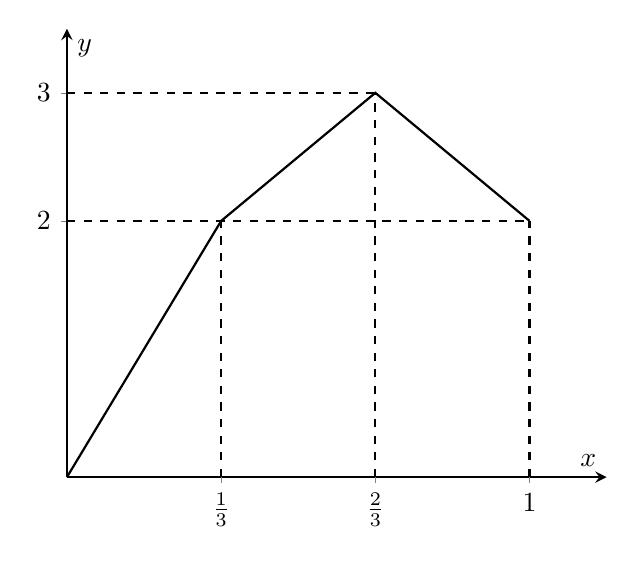
\begin{tikzpicture}
      \begin{axis}[
          axis lines=middle, 
          xticklabels={},
          xtick={1,...,3},
          ytick={2,...,3},
          extra x ticks={1,2,3},
          extra x tick labels={$\frac{1}{3}$,$\frac{2}{3}$,$1$},
          xmin=0, xmax=3.5,
          ymin=0, ymax=3.5,
          xlabel={$x$}, ylabel={$y$},
          samples=200,
          %domain=0:1,
          thick
      ]
      \addplot[no marks] table {
        x   y
        0   0
        1   2
        2   3
        3   2
        };
      \addplot[no marks,dashed] table {
        x y
        0 2
        3 2
        };
      \addplot[no marks,dashed] table {
        x y
        0 3
        2 3
        };
      \addplot[no marks,dashed] table {
        x y
        1 0
        1 2
        };
      \addplot[no marks,dashed] table {
        x y
        2 0
        2 3
        };
      \addplot[no marks,dashed] table {
        x y
        3 0
        3 2
        };
    \end{axis}
  \end{tikzpicture}
\end{figure}

\newpage
\subsection{Tvrzení o kladnosti komponent matice \texorpdfstring{$A$}{A}}
Nechť $E \in \M_{m,n} (\R)$ je matice samých jedniček $\left(\text{tj. } E = 
\begin{bmatrix}
    1 & 1 & \dots & 1 \\
    \vdots & \vdots &  & \vdots \\
    1 & 1 & \dots & 1
\end{bmatrix}\right)$, $v \in \R$ je cena hry $\Gamma(A)$ a $c \in \R$. 
Potom $\O_1(A) = \O_1(A + cE)$, $\O_2(A) = \O_2(A + cE)$ a cena hry $\Gamma(A+cE)$ je $v+c$.

Důkaz.

Vezměme si
\begin{align*}
    \hat x \in \O_1(A) &\text{ a } \hat y \in \O_2(A) \\
    & \Big\Updownarrow \\
   \langle A \hat y, x\rangle \leq \langle A &\hat y, \hat x\rangle \leq \langle Ay, \hat x\rangle 
   \quad \forall x \in X \, \forall y \in Y
\end{align*}
Tedy $(\hat x, \hat y)$ je \hyperref[sedl]{sedlový bod}, kde $f$ z definice je funkce úžitku, která je dána skalárním 
součinem.
\begin{align*}
    & \Big\Updownarrow \\
    \langle A \hat y, x\rangle + c \leq \langle A \hat y, \, \hat x\rangle + c &\leq \langle Ay, \hat x\rangle + c
    \quad \forall x \in X \, \forall y \in Y \\
    & \Big\Updownarrow \langle Ey, x\rangle = \left\langle \begin{bmatrix}1 \\ \vdots \\ 1\end{bmatrix}, x\right\rangle
    = 1 \quad \forall x \in X \, \forall y \in Y \\
    \langle A \hat y, x\rangle + c \langle E \hat y, x\rangle \leq \langle A \hat y, \hat x\rangle &+ c 
    \langle E \hat y, \hat x\rangle \leq \langle Ay, \hat x\rangle + c \langle Ey, \hat x\rangle 
    \quad \forall x \in X \, \forall y \in Y \\
    & \Big\Updownarrow \text{ linearita} \\
    \langle (A + cE)\hat y, x\rangle \leq \langle (A+cE)\hat y, \hat x\rangle &\leq \langle (A+cE)y, \hat x\rangle
    \quad \forall x \in X \, \forall y \in Y
\end{align*}
Což je nutně ekvivalentní s
\[
    \hat x \in \O_1(A+cE), \, \hat y \in \O_2(A+cE).
\]
Cena hry $\Gamma(A+cE)$ je
\[
    \langle (A+cE)\hat y, \hat x\rangle = \underbrace{\langle A \hat y, \hat x\rangle}_{=v} + 
    c \underbrace{\langle E \hat y, x\rangle}_{=1} = v + c. \qed
\]

\subsection{Souvislost maticové hry a lineárního programování}
Množina $\O_1(A)$ je množina všech řešení úlohy
\[
\left.\begin{aligned}
    &\text{maximalisujte}&& \min_{j \in \bc{1, \dots, n}} \langle A f_j, x\rangle \\
    &\text{za podmínky}  && \sum_{i=1}^{m}x_i = 1, \\
    &\phantom{\text{za podmínky}}&&x \geq 0.
\end{aligned}
\right\} (U1)
\]
Množina $\O_2(A)$ je množina všech řešení úlohy
\[
\left.\begin{aligned}
    &\text{minimalisujte}&& \max_{i \in \bc{1, \dots, m}} \langle A y, e_i\rangle \\
    &\text{za podmínky}  && \sum_{j=1}^{n}y_j = 1, \\
    &\phantom{\text{za podmínky}}&&y \geq 0.
\end{aligned}
\right\} (U2)
\]
Takové úlohy ale můžeme přepsat (například přepišme $U1$):
\[
\begin{aligned}
    &\text{maximalisujte}&& w \\
    &\text{za podmínky}  && \min_{j \in {1, \dots, n}} \geq w, \\
    &\phantom{\text{za podmínky}}&&\sum_{i=1}^{m} x_i = 1, \\
    &\phantom{\text{za podmínky}}&& x \geq 0.
\end{aligned}
\]
Což ale stále jde přepsat:
\[
\begin{aligned}
    &\text{maximalisujte}&& w \\
    &\text{za podmínky}  && \langle A f_j, x\rangle \geq w \quad \forall j \in \bc{1, \dots, n}, \\
    &\phantom{\text{za podmínky}}&&\sum_{i=1}^{m} x_i = 1, \\
    &\phantom{\text{za podmínky}}&& x \geq 0.
\end{aligned}
\]
Můžeme uvážit jen $w >0$, neboť $A$ má všechny komponenty kladné 
(tj. $\langle Af_j, x\rangle > 0 \quad \forall j$). 
\[
\begin{aligned}
    &\text{minimalisujte}&& \frac{1}{w} \\
    &\text{za podmínky}  && \left\langle A f_j, \frac{x}{w}\right\rangle \geq 1 \quad \forall j \in \bc{1, \dots, n}, \\
    &\phantom{\text{za podmínky}}&&\sum_{i=1}^{m} \frac{x_i}{w} = \frac{1}{w}, \\
    &\phantom{\text{za podmínky}}&& \frac{x}{w} \geq 0,
    &\phantom{\text{za podmínky}}&& w \geq 0.
\end{aligned}
\]
Označme si $\1_k = (1, \dots, 1)^T \in \R^k$. Také uvažme substituci $\xi = \frac{x}{w}$.
\[
    \sum_{i=1}^{m} \frac{x_i}{w} = \frac{1}{w} = \langle \frac{x}{w}, \frac{1}{w}\rangle
\]
Tudíž konečně
\[
\begin{aligned}
    &\text{minimalisujte}&& \langle \xi, \1_k\rangle \\
    &\text{za podmínky}  && \left\langle A f_j, \xi\right\rangle \geq 1 \quad \forall j \in \bc{1, \dots, n}, \\
    &\phantom{\text{za podmínky}}&&\xi \geq 0.
\end{aligned}
\]
což je krásná úloha lineárního programování.

Můžeme ještě přepsat na maticový zápis
\[
\left.\begin{aligned}
    &\text{minimalisujte}&& \langle \xi, \1_k\rangle \\
    &\text{za podmínky}  && A^T \xi \geq \1_n, \\
    &\phantom{\text{za podmínky}}&&\xi \geq 0.
\end{aligned}
\right\} (P)
\]

Stejným postupem získáme i přepis $U2$.
\[
\left.\begin{aligned}
    &\text{maximalisujte}&& \langle \eta, \1_k\rangle \\
    &\text{za podmínky}  &&  A \eta \leq \1_m, \\
    &\phantom{\text{za podmínky}}&&\eta \geq 0.
\end{aligned}
\right\} (D)
\]
Pozorování. Úlohy jsou vzájemně duální.

\subsection{Příklad na vztah maticové hry a LP}
Je dána hra $\Gamma(A)$ s maticí hry
\[
    A = 
    \begin{bmatrix}
        3 & 1 & 5 \\
        2 & 4 & 3    
    \end{bmatrix}.
\]
Jaká je optimální strategie 1. a optimální strategie 2. hráče?

Matice $A$ už má všechny komponenty kladné, tudíž nemusíme přičítat nějakou konstantu $c$.
\begin{multicols}{2}
    \[
    \begin{aligned}
        &\text{minimalisujte}&& \xi_1 + \xi_2 \\
        &\text{za podmínky}  && 
        \begin{bmatrix}
            3 & 2 \\
            1 & 4 \\
            5 & 3
        \end{bmatrix}
        \begin{bmatrix}
            \xi_1 \\ \xi_2
        \end{bmatrix} \geq 
        \begin{bmatrix}
            1 \\ 1 \\ 1
        \end{bmatrix}, \\
        &\phantom{\text{za podmínky}}&&\xi \geq 0.
    \end{aligned}
    \]

    \[
    \begin{aligned}
        &\text{maximalisujte}&& \eta_1 + \eta_2 + \eta_3 \\
        &\text{za podmínky}  && 
        \begin{bmatrix}
            3 & 1 & 5 \\
            2 & 4 & 3
        \end{bmatrix}
        \begin{bmatrix}
            \eta_1 \\ \eta_2 \\ \eta_3
        \end{bmatrix} \leq 
        \begin{bmatrix}
            1 \\ 1
        \end{bmatrix}, \\
        &\phantom{\text{za podmínky}}&&\eta \geq 0.
    \end{aligned}
    \]
\end{multicols}
Vybereme si jednu z těchto úloh, ideálně tu jednodušší. Tou bude druhá, tedy maximalisační, úloha.
\[
    \begin{array}{cccccc|c}
        &\eta_1 & \eta_2 & \eta_3 & \eta_4 & \eta_5 & \\
        &-1 & -1 & -1& 0 & 0 & 0 \\ \hline
        \eta_4 &\phantom{-}\Rnode{C}{3}  & \phantom{-}1  & \phantom{-}5 & 1 & 0 & \Rnode{B}{1} \\
        \eta_5 &\phantom{-}\Rnode{A}{2}  & \phantom{-}4  & \phantom{-}3 & 0 & 1 & 1  \\
    \end{array}
    \psset{linewidth=1pt, linearc=0.1, linecolor=red, boxsize=0.5em}
    \ncbox[nodesep=0.2em]{A}{C}\ncbox[nodesep=0.3ex]{C}{B}
\]
\[
    \begin{array}{cccccc|c}
        &\eta_1 & \eta_2 & \eta_3 & \eta_4 & \eta_5 & \\
        &0 & -\frac{2}{3} & \phantom{-}\frac{2}{3}& \phantom{-}\frac{1}{3} & 0 & \frac{1}{3} \\ \hline
        \eta_1 &1 & \phantom{-}\Rnode{C}{\frac{1}{3}} & \phantom{-}\frac{5}{3} & \phantom{-}\frac{1}{3} & 0 & \frac{1}{3} \\
        \eta_5 &0 & \phantom{-}\Rnode{A}{\frac{10}{3}} & -\frac{1}{3} & -\frac{2}{3} & 1 & \Rnode{B}{\frac{1}{3}} \\
    \end{array}
    \psset{linewidth=1pt, linearc=0.1, linecolor=red, boxsize=0.5em}
    \ncbox[nodesep=0.2em]{A}{C}\ncbox[nodesep=0.3ex]{A}{B}
\]
\[
    \begin{array}{cccccc|c}
        &\eta_1 & \eta_2 & \eta_3 & \eta_4 & \eta_5 & \\
        &0 & 0 & \frac{2}{3} - \frac{2}{30}& \frac{1}{3}-\frac{4}{30} & \frac{2}{10} & \frac{1}{3}+\frac{2}{30} \\ \hline
        \eta_1 &1  &0  & x & x & x & \frac{1}{3}-\frac{1}{30} \\
        \eta_2 &0  & 1  & -\frac{1}{10} & -\frac{2}{10} & \frac{3}{10} & \frac{1}{10}  \\
    \end{array}
\]
A tedy: $\eta_1 = \frac{9}{30} = \frac{3}{10}$, $\eta_2 = \frac{1}{10}$, $\eta_3 = 0$.
\[\xi_1 = \frac{6}{30} = \frac{1}{5}, \xi_2 = \frac{1}{5}\]
\begin{align*}
    \implies \hat x &= \frac{1}{2}\begin{bmatrix} 1 \\ 1\end{bmatrix} \\
    \hat y &= \frac{1}{4}\begin{bmatrix} 3 \\ 1 \\ 0\end{bmatrix}
\end{align*}

